\documentclass[12pt,twoside]{scrartcl}
\usepackage[a4paper,top=2cm,left=2cm,right=2cm,bottom=2cm,includefoot,includehead]{geometry}
\usepackage{graphicx}
\usepackage[numbers]{natbib} % Add this line for natbib package
\usepackage{fancyhdr}
\usepackage{hyperref}
\usepackage{amsmath}
\graphicspath{ {figures/} }



\pagestyle{fancy} % Set the page style to fancy
\fancyhf{} % Clear all header and footer fields

% Define the header and footer content for odd and even pages
\fancyhead[CE,CO]{School of Electrical Engineering} % Left header on even pages, right header on odd pages
% \fancyhead[RE,LO]{Right Header} % Right header on even pages, left header on odd pages
\fancyfoot[LE,RO]{\thepage} % Page number on left footer of even pages and right footer of odd pages
\fancyfoot[RE,LO]{ELEC3251} % Left footer on odd pages, right footer on even pages

\begin{document}
\pagenumbering{arabic}
\setcounter{page}{1}
\begin{titlepage}
    \begin{center}

        
\includegraphics[width=0.2\textwidth]{LOGO_Square.pdf}

        \vspace*{0.4cm}
        School of Electrical Engineering \\
        University of Newcastle
        
        \vspace{1cm}
        \huge
        \textbf{\textsf{ELEC3251 \\ Assignment 1}}

        \vspace{0.5cm}
        \large
        \textbf{\textsf{Practical and Theoretical Analysis of \\ Buck Converter and Flyback Converter}}

        \vspace{1.5cm}
        \normalsize
        \begin{tabular}{l|r}
            Liam Patey-Dennis & c3349900 \\
            Joshua Thomas & c3376353
        \end{tabular}
        \vfill    
    \end{center}
\end{titlepage}


\section{Buck Converter}
\subsection{Ideal Calculations}
The duty cycle required to achieve an output voltage of $V_{o} = 5$ V for an input supply voltage of $V_{d} = 12$ V can be determined using the DC transfer function of the Buck converter, see Equation \ref{equation:Buck_TF}. The resulting duty cycle required for the ideal circuit is $D \approx 41.67$\%.\par
\begin{equation}
\frac{V_o}{V_d} = D \label{equation:Buck_TF}
\end{equation}
The output voltage ripple ($\Delta V_o$) of an ideal Buck converter is given by Equation \ref{equation:Buck_ripple}. This equation can be rearranged, see Equation \ref{equation:Buck_cap}, to find the required capacitance for the low pass filter, provided that the duty cycle ($D$), filter inductance ($L$), and switching period ($T_{s}$) are known. For $T_{s} = 1/f_{s} = 10$ $\mu$s, $L = 1$ mH, $D = 41.67$\%, $\Delta V_{o} = 25$ mV, and $V_o = 5$ V, the required capacitance is $C = 1.458$ $\mu$F. \par
\begin{equation}
\frac{\Delta V_{o}}{V_{o}} = \frac{1}{8}\frac{T_{s}^{2}(1-D)}{LC} \label{equation:Buck_ripple}
\end{equation}
\begin{equation}
C = \frac{V_o}{\Delta V_{o}}\frac{T_{s}^{2}(1-D)}{8L} \label{equation:Buck_cap}
\end{equation}
The output power of the converter will be limited by the ratings of the components in the circuit. As the output voltage of the converter is required to remain constant at $5$ V, only the output current can be adjusted to suit the ratings of the components. The inductor selected for the circuit is the Murata \#1410516C, which has a maximum DC current of $1.6$ A \cite{RNX0}. A IRFZ24NPbF MOSFET has been selected for the switch, this component has a maximum DC current rating of $17$ A \cite{RNX1}. The selected diode is an SB120 which has a maximum DC current of $1.0$ A \cite{RNX2}. The inductor current will equal the output current, assuming the voltage across the capacitor remains constant. Therefore, the output current must be less than $1.6$ A, to avoid causing damage to the inductor. The diode will only conduct when the switch is off, therefore the DC current flowing through the diode is $I_{D} = (1-D)I_{o}$. For $I_{o} = 1.6$ A the diode current is $0.93$ A, which is less than the maximum rating of the device. Therefore, the load resistance must be selected such that $I_{o} \le 1.6$ A. Using Ohm’s law this inequality is equivalent to $R_{Load} \ge 3.125$ $\Omega$. The smallest resistor provided in the laboratory kit is $3.9$ $\Omega$ so this resistance will be used for the load.\par
\vspace{5mm}
\noindent The continuous conduction mode (CCM) and discontinuous conduction mode (DCM) boundary occurs when the current flowing through the inductor reaches $0$ A. For the ideal Buck converter this will occur for a DC output current ($I_{oB}$) which can be found using Equation \ref{equation:Buck_DCM}. For the designed converter the minimum DC output current is $I_{oB} = 14.6$ mA, which is equivalent to an output load of $342$ $\Omega$.
\begin{equation}
I_{oB} \approx \frac{T_{s}V_{o}}{2L}(1-D) \label{equation:Buck_DCM}
\end{equation}
\pagebreak
\subsection{Ideal Simulations}
Wolfram System Modeller (Wolfram) was used to simulate the performance of the designed converter. The model used for the simulations is shown in Figure \ref{fig:Buck_idealModel}. The output voltage of the ideal Buck converter is shown in Figure \ref{fig:Buck_idealVout}. The RMS output voltage is 4.9983 V, which lies close to the theoretically expected value of 5 V. The slight discrepancy between the simulated value and the expected value may be the result of truncating the duty cycle to 4 decimal places ($5/12 \approx 0.4167$). It may also be a result of the numerical methods used by the Wolfram software to simulate the system. An output voltage ripple of 6.67 mV is observed. This ripple is smaller than the expected ripple of 25 mV, this may be the result of the assumption that the output ripple is independent of the load impedance. The addition of the load resistance results in an RLC filter at the output of the converter. This resistance dampens the resonant peak of the LC combination which is likely to result in larger amounts of attenuation for the high frequency components of the output voltage.\par
\vspace{5mm}
\noindent Figure \ref{fig:buck_DCM} (A) displays the inductor current for a load resistance of 342 $\Omega$. The current reaches a minimum value of $120 $ $\mu$A, which indicates that the converter is close to the CCM-DCM boundary. Figure \ref{fig:buck_DCM} (b) displays the current for a load resistance of 345 $\Omega$. Slight distortion is observed in the waveform near the zero crossing which indicates that the converter has entered DCM. This suggests that the CCM-DCM boundary lies in the range $342 \le R_{Load} \le 345$ $\Omega$ which agrees with the theoretically expected value of 342 $\Omega$. The boundary may not lie exactly at 342 $\Omega$ because of the assumption, made in Equation \ref{equation:Buck_DCM}, that the inductor current and the output current are equal. This assumption is not correct as a small amount of current also flows through the capacitor.

\begin{figure}[h]
    \centering
    \includegraphics[width=0.7\textwidth]{Buck_idealModel}
    \caption{Modelica model used to simluate the operation of the ideal Buck converter.}
    \label{fig:Buck_idealModel}
\end{figure}

\begin{figure}[h]
    \centering
    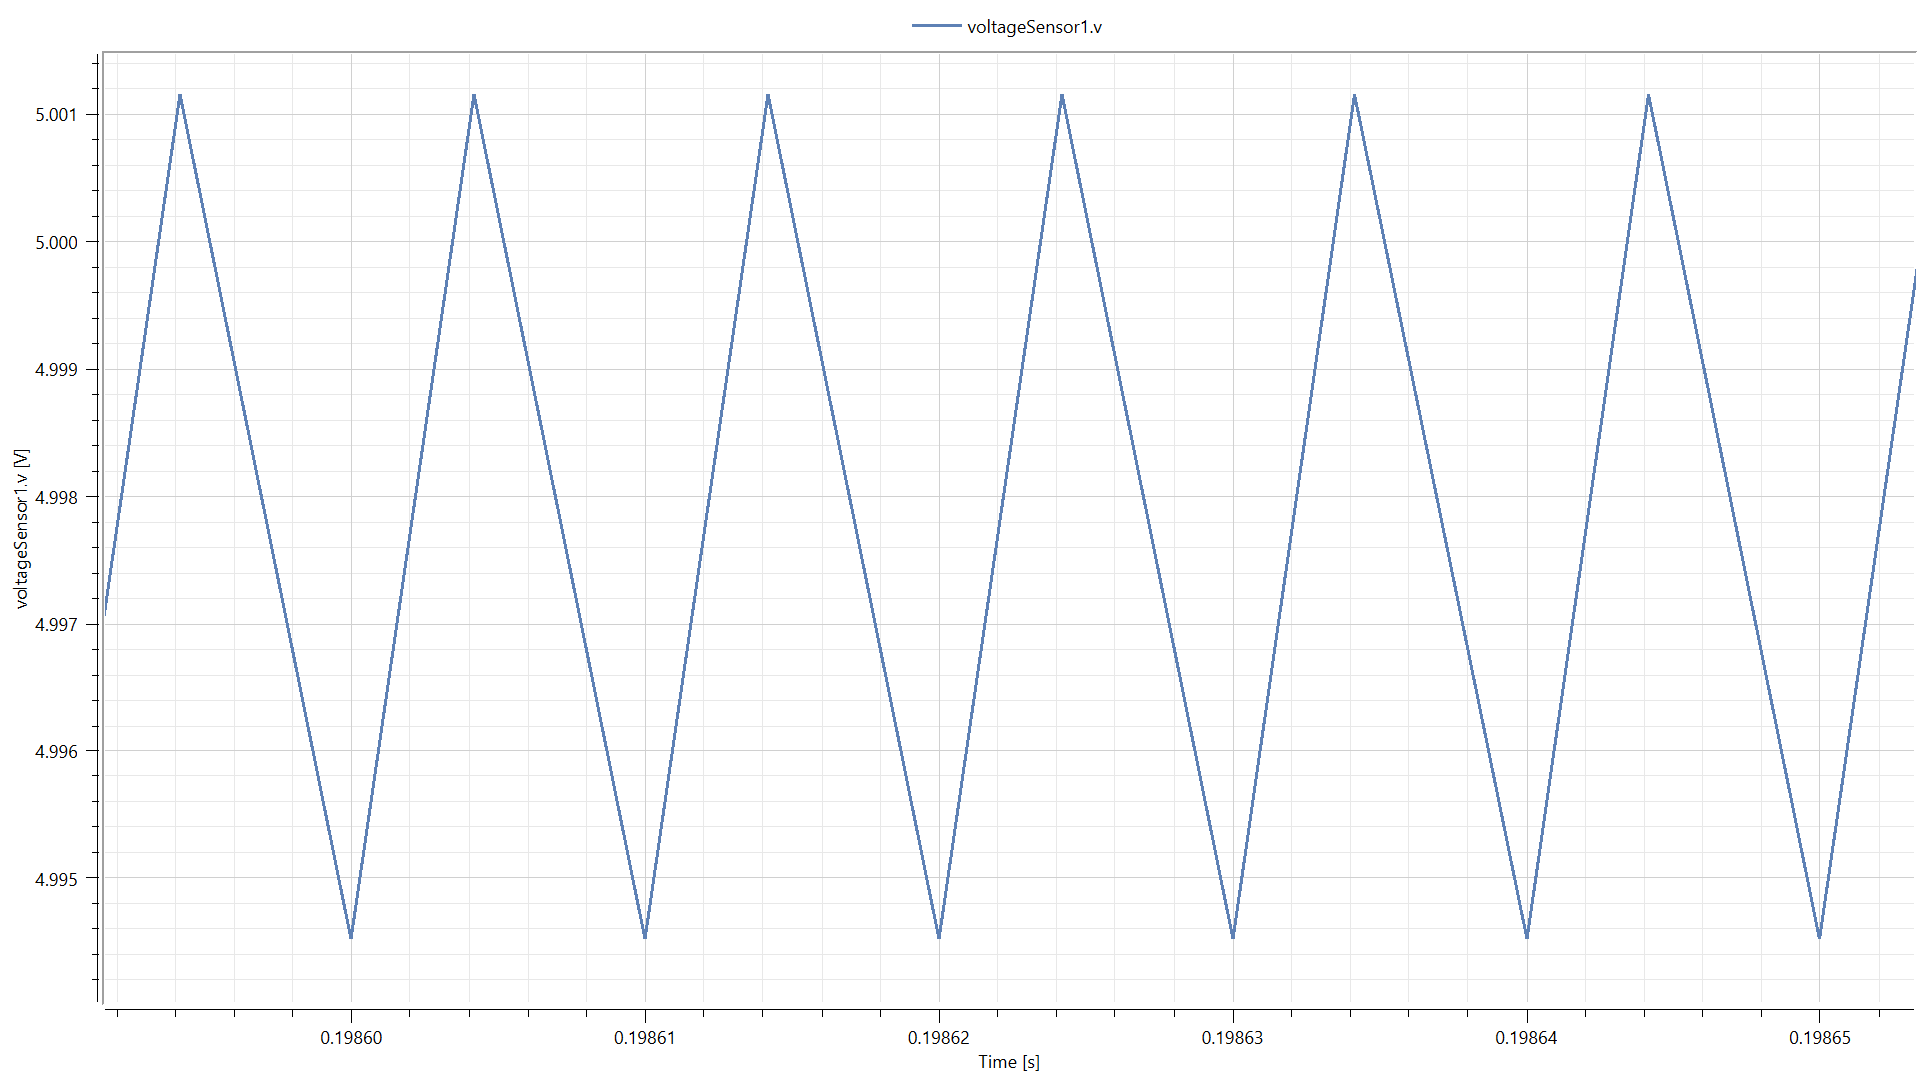
\includegraphics[width=0.6\textwidth]{Buck_idealVout}
    \caption{Ideal Buck converter output voltage in steady state. An RMS value of 4.9983 V and a voltage ripple of 6.67 mV are observed.}
    \label{fig:Buck_idealVout}
\end{figure}

\begin{figure}[h!]
    \centering
    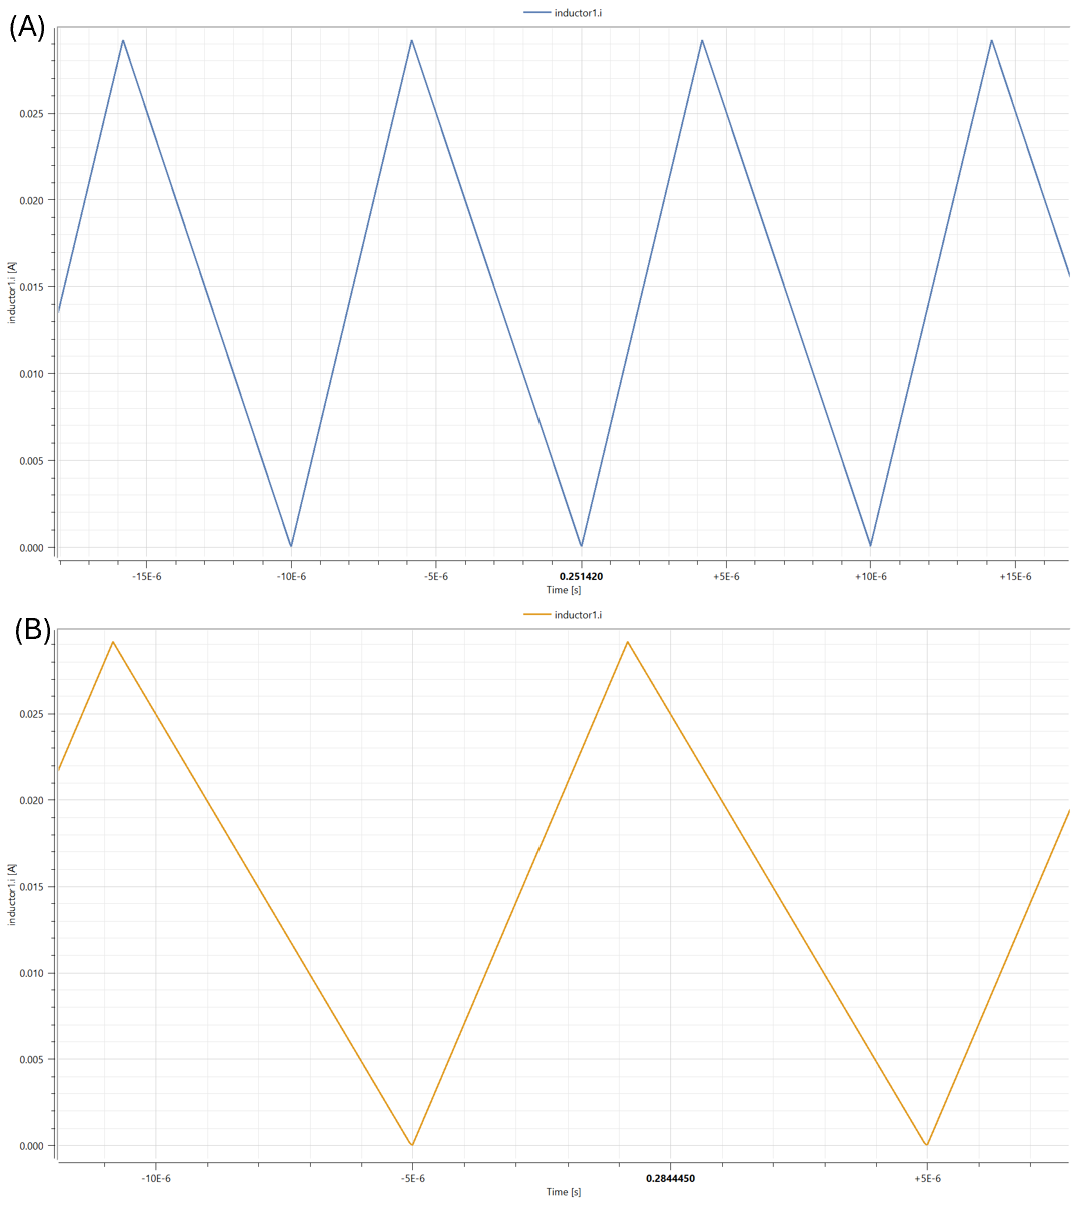
\includegraphics[width=0.6\textwidth]{buck_DCM}
    \caption{Buck converter inductor current for a load resistance of (A) 342 $\Omega$, and (B) 345 $\Omega$. A small amount of distortion is present in (B) which indicates that the CCM-DCM boundary lies in the range $342 \le R_{Load} \le 345$ $\Omega$.}
    \label{fig:buck_DCM}
\end{figure}
\newpage

\subsection{Non Ideal Calculations}
The previous calculations and simulations neglect many real-world effects that will affect the circuit's performance. Previously, no voltage losses were assumed to occur across the switch. This assumption is invalid as all switches have non-zero on resistances. Furthermore, it was assumed that no voltage drop occurs across the diode. All diodes have a non-zero voltage drop, which is required to overcome the potential barrier formed at the P-N junction of these devices. In addition, the windings of an inductor are not perfect conductors and hence have resistance. These effects will result in the output voltage of the converter being lower than the theoretically expected value. Figure \ref{fig:Buck_nonIdealCircuits} displays equivalent circuit models which can be used to account for these effects when (A) the switch is on and (B) when the switch is off. Applying Kirchoff’s voltage law (KVL) to the outer loop of each circuit, results in Equations \ref{equation:KVL_on} and \ref{equation:KVL_off}.
\begin{equation}
V_{L,on} = V_{d} - V_{o} - V_{loss, on} = V_{d} - V_{o} - (R_{DS}+ R_{L})i_{L} \label{equation:KVL_on}
\end{equation}
\begin{equation}
V_{L,off} = -V_{o} - V_{f} - V_{loss, off} = V_{o} - V_{f} - R_{L}i_{L}\label{equation:KVL_off}
\end{equation}
Where $R_{DS}$ is the on resistance of the switch, $R_{L}$ is the inductor resistance, and $V_{f}$ is the forward voltage of the diode.\par
\vspace{5mm}
\noindent If it is assumed that the circuit is in steady state, then the zero volt-seconds assumption can be applied which yields,
\begin{equation*}
V_{L,on}t_{on} + V_{L,off}t_{off} = 0
\end{equation*}
If the inductor current is assumed to be equal to the load current then,
\begin{equation*}
i_{L} \approx i_{Load} = \frac{V_{o}}{R_{Load}}
\end{equation*}
Which can be used with the previous equation to obtain Equation \ref{equation:Buck_nonIdealTF}.
\begin{align}
V_{o} &= \frac{R_{Load}}{(1+2D)R_{Load} - R_{L} - DR_{DS}}\left\{DV_{d} - (1-D)V_{f} \label{equation:Buck_nonIdealTF}\right\}
\end{align}
\noindent For the ideal duty cycle ($D = 41.67$\%) with the parameters $R_{DS} = 0.07$ $\Omega$, $R_{L} = 1.6$ $\Omega$, $V_{f} = 0.7$ V and a load current of $i_{L} = 1.28$ A ($R_{Load} = 3.9$ $\Omega$), the expected output voltage of the converter is $V_{o} =3.24$ V \cite{RNX1, RNX0, RNX2}. The duty cycle required to obtain an output of 5 V is $D = 61.44$\%.\par
\vspace{5mm}
\noindent The CCM-DCM boundary occurs when the output current is approximately equal to half of the peak current through the inductor. The peak current through the inductor is given by Equation \ref{equation:buck_iPeak}.\par
\begin{equation}
i_{pk} = \frac{1}{L}\int_{0}^{t_{on}}v_{L} \,dt \label{equation:buck_iPeak}
\end{equation}
\noindent For the ideal case the voltage across the inductor (when the switch is on) is:
\begin{equation*}
v_{L,ideal} = V_{d} - V_{o}
\end{equation*}
For the non-ideal case the voltage is:
\begin{equation*}
v_{L,non-ideal}(t) = V_{d} - V_{o} - i_{L}(t)(R_{DS} + R_{L})
\end{equation*}
Where,
\begin{equation*}
v_{L,ideal} \ge v_{L,non-ideal}(t)
\end{equation*}
Which implies,
\begin{align*}
i_{pk,ideal} &> i_{pk,non-ideal} \\
\intertext{Thus,}
 I_{oB,ideal} &> I_{oB,non-ideal}
\end{align*}
Therefore, it is expected that a larger load resistance will be required for the non-ideal Buck converter, to observe the CCM-DCM boundary.\par

\newpage
\subsection{Non Ideal Simulations}
Figure \ref{fig:Buck_nonIdealModel} displays the Modelica model used to perform the non-ideal simulation. The non ideal switch model from the \textit{InverterParts}.\textit{NonIdeal\_Components} library was used to replicate the IRFZ24NPbF MOSFET. The reverse diode voltage (1.3 V), series resistance (0.07 $\Omega$), parallel resistance (2 M$\Omega$), turn on time (4.9 ns), and turn off time (19 ns) of the MOSFET are included in this model. The 1.6 $\Omega$ resistor is used to model the series resistance of the inductor and the $1.3\times10^{-11}$ F capacitor is used to model the self-resonant frequency of the inductor. The non ideal diode model from the \textit{InverterParts}.\textit{NonIdeal\_Components} library was used to replicate the SB120 diode. The worst case forward voltage (0.70 V) and the junction capacitance (110 pF) of the SB120 were included in this model. An output capacitance of 1 $\mu$F has been used in the simulation. This capacitance was selected as it lies close to the theoretically predicted value and was the largest capacitance that can be achieved with the laboratory kit without placing multiple capacitors in series. \par
\vspace{5mm}
\noindent The output voltage of the non-ideal converter for the ideal duty cycle is shown in Figure \ref{fig:buck_NI_output_oldD}. An RMS voltage of 3.2164 V is observed, which lies close to the theoretically predicted value of 3.24 V. The slight deviation from this value may be the result of assuming that the output current is constant and equal to the current through the inductor. Figure \ref{fig:buck_NI_output_newD} displays the output voltage for a duty cycle of 61.44\%, an RMS voltage of 5.0010 V is observed which lies close the predicted value. A ripple voltage of 27.739 mV is observed which lies close to the specified value of 25 mV. The increase in the voltage ripple for the non-ideal simulation is likely a result of the reducing the size of the output capacitor, increasing the duty cycle, and including the parasitic capacitance of the inductor. This ripple could be reduced through increasing the size of the output capacitor.\par
\begin{figure}[h]
    \centering
    \includegraphics[width=0.7\textwidth]{Buck_nonIdealModel}
    \caption{Modelica model used to simluate the operation of the non ideal Buck converter.}
    \label{fig:Buck_nonIdealModel}
\end{figure}

\begin{figure}[h]
    \centering
    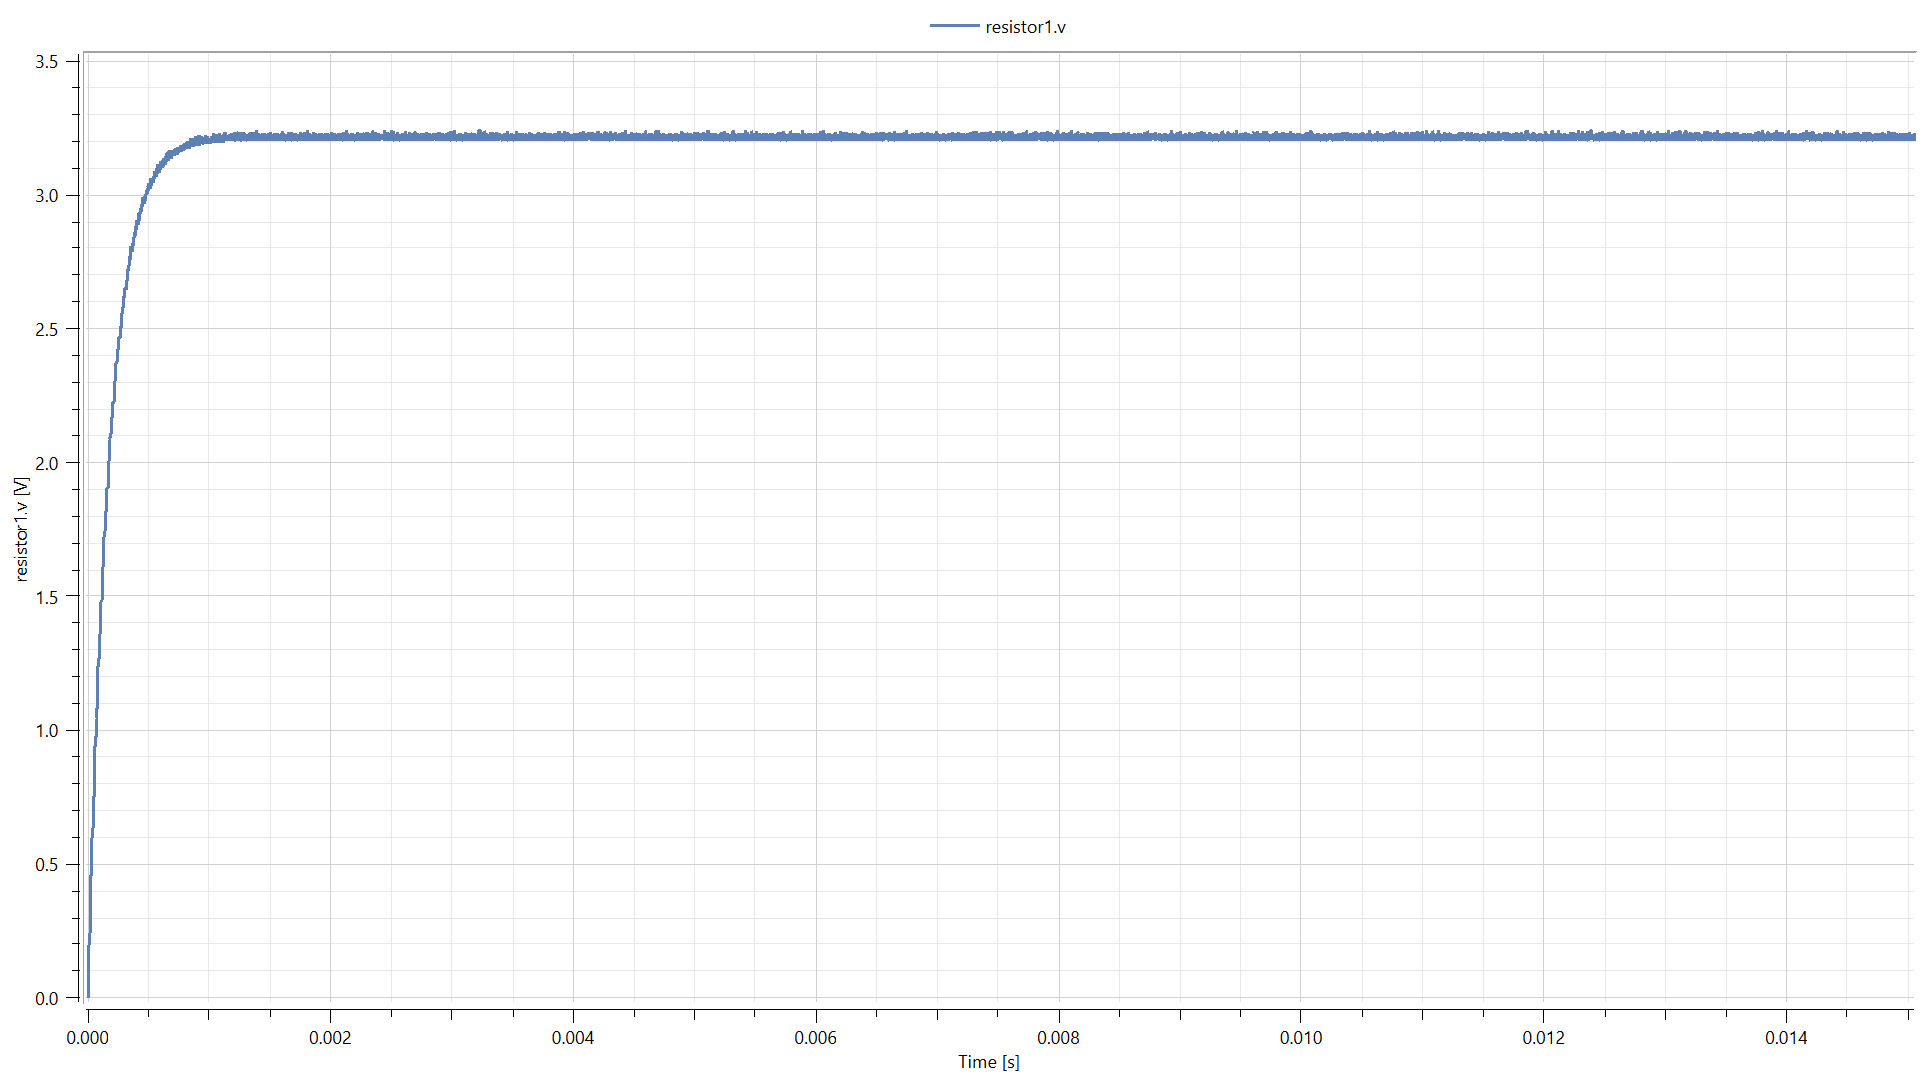
\includegraphics[width=0.6\textwidth]{buck_NI_output_oldD}
    \caption{Non-ideal Buck converter output voltage for duty cycle of 41.67\% and a load of $3.9$ $\Omega$. An average voltage of 3.2164 V is observed.}
    \label{fig:buck_NI_output_oldD}
\end{figure}
\begin{figure}[h]
    \centering
    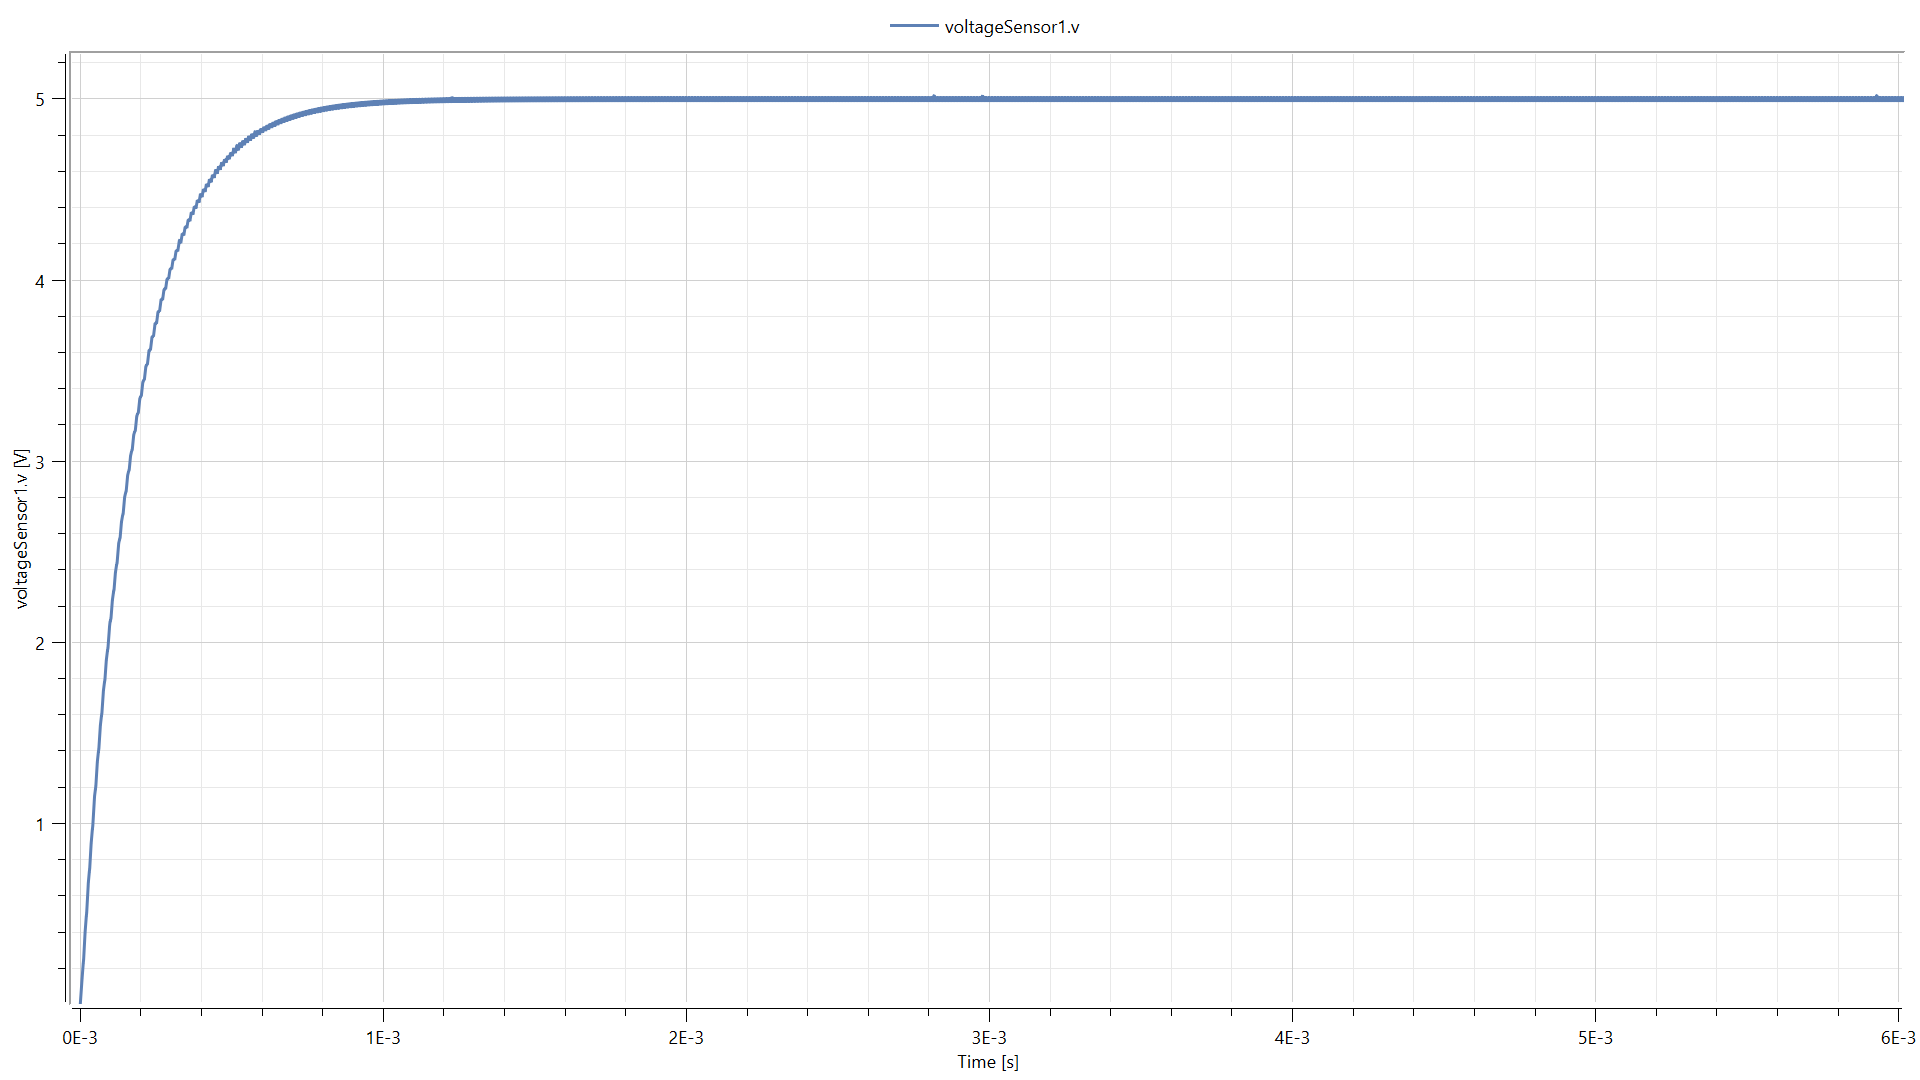
\includegraphics[width=0.6\textwidth]{buck_NI_output_newD}
    \caption{Non-ideal Buck converter output voltage for duty cycle of 61.44\% and a load of $3.9$ $\Omega$. An average voltage of 5.0010 V and a ripple voltage of 27.739 mV is observed.}
    \label{fig:buck_NI_output_newD}
\end{figure}
\pagebreak

\noindent The current through the inductor for $D = 61.44$\% (rated power conditions) is shown in Figure \ref{fig:buck_Current}. An RMS current of 1.2847 A is observed which matches the theoretically predicted value and does not exceed the maximum ratings of the devices. The inductor current for a load of (A) 470 $\Omega$ and (B) 475 $\Omega$ is shown in Figure \ref{fig:buck_NIDCM}. The inductor current for the 475 $\Omega$ passes through the 0 A crossing for a period of time. This indicates that the circuit has entered DCM. The 470 $\Omega$ load results in a current which gets close to the 0 A crossing. Therefore the load resistance for the CCM-DCM boundary is expected to lie in the range $470 \le R_{Load} \le 475$ $\Omega$. \par
\newpage

\begin{figure}[h]
    \centering
    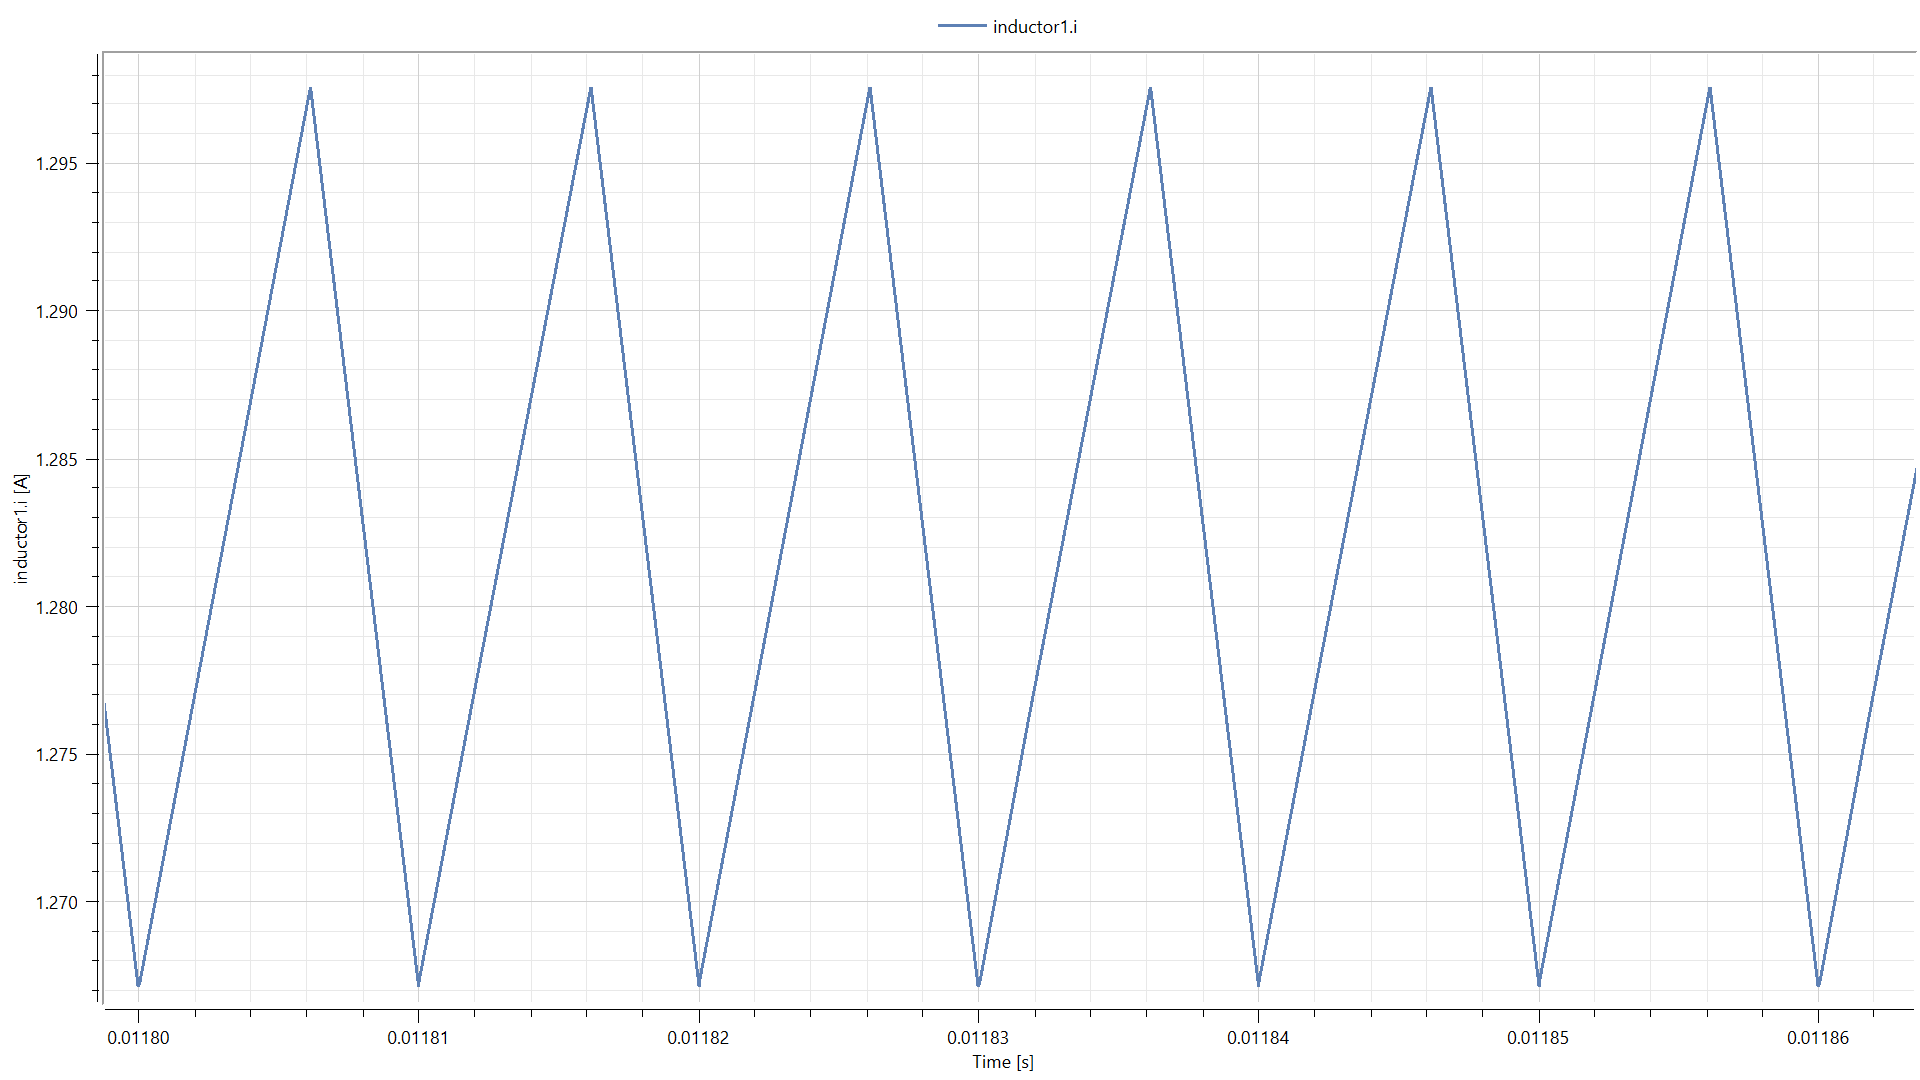
\includegraphics[width=0.6\textwidth]{buck_Current}
    \caption{Inductor current for the non ideal Buck converter under rated power conditions.}
    \label{fig:buck_Current}
\end{figure}

\begin{figure}[h!]
    \centering
    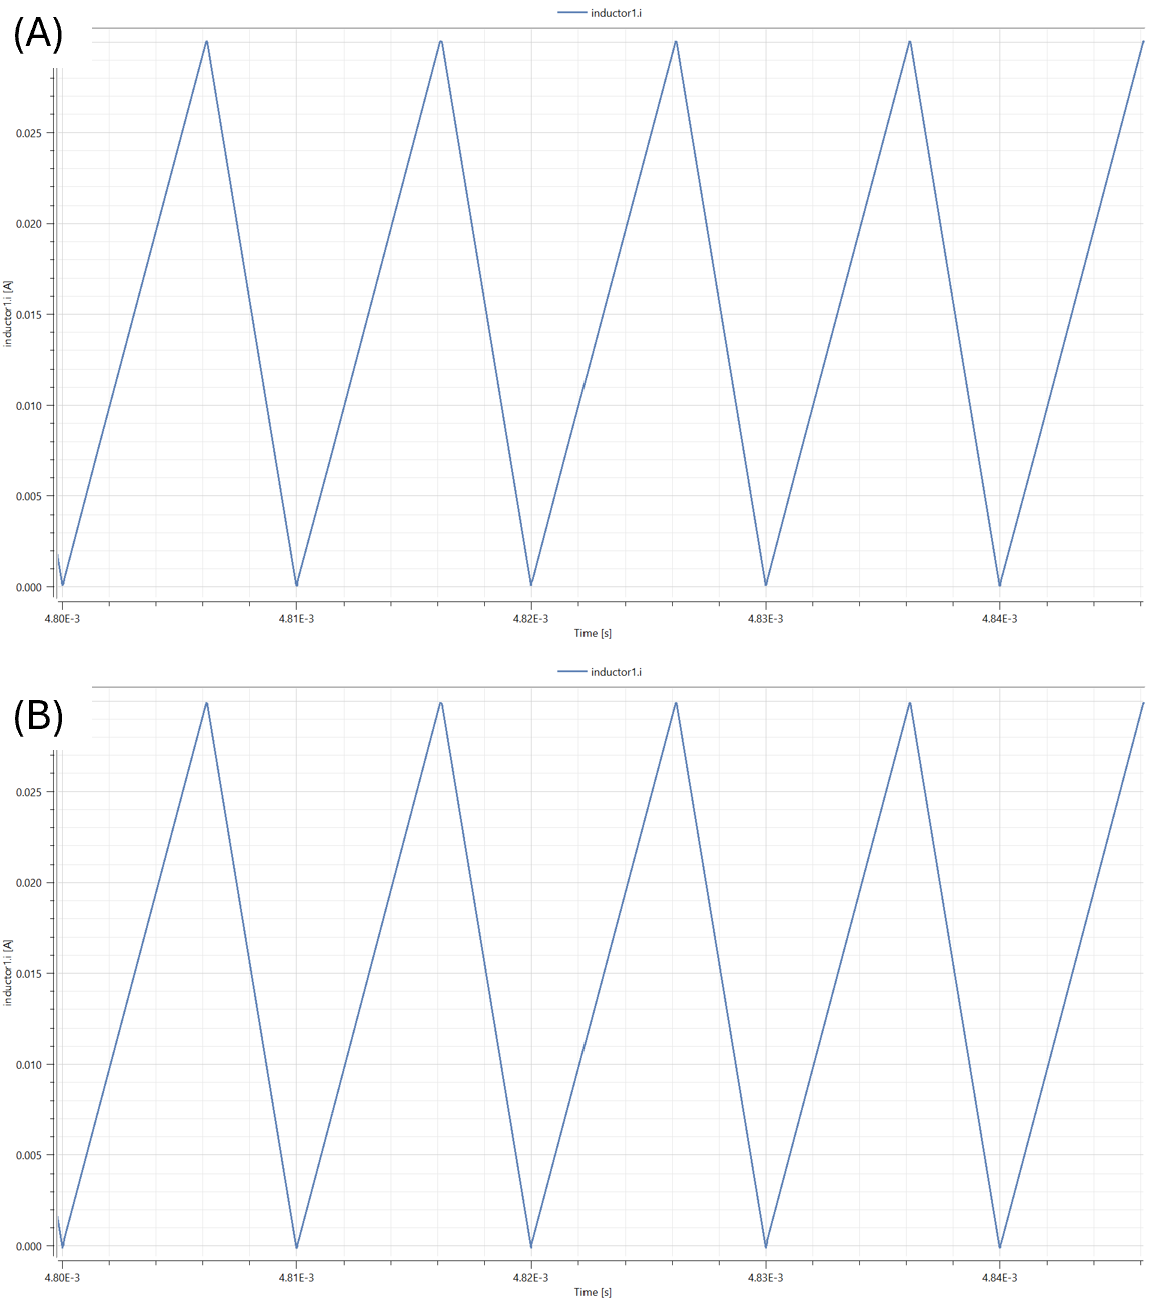
\includegraphics[width=0.6\textwidth]{buck_NIDCM}
    \caption{Inductor current for the non ideal Buck converter under rated power conditions.}
    \label{fig:buck_NIDCM}
\end{figure}

\subsection{Results}
The constructed Buck converter is shown in Figure \ref{fig:buck_real}. The circuit was constructed on a breadboard and multicore twisted wires were used. The PWM input signal for the gate driver was generated using a signal generator and the output voltage was monitored using an oscilloscope. \par

\begin{figure}[h]
    \centering
    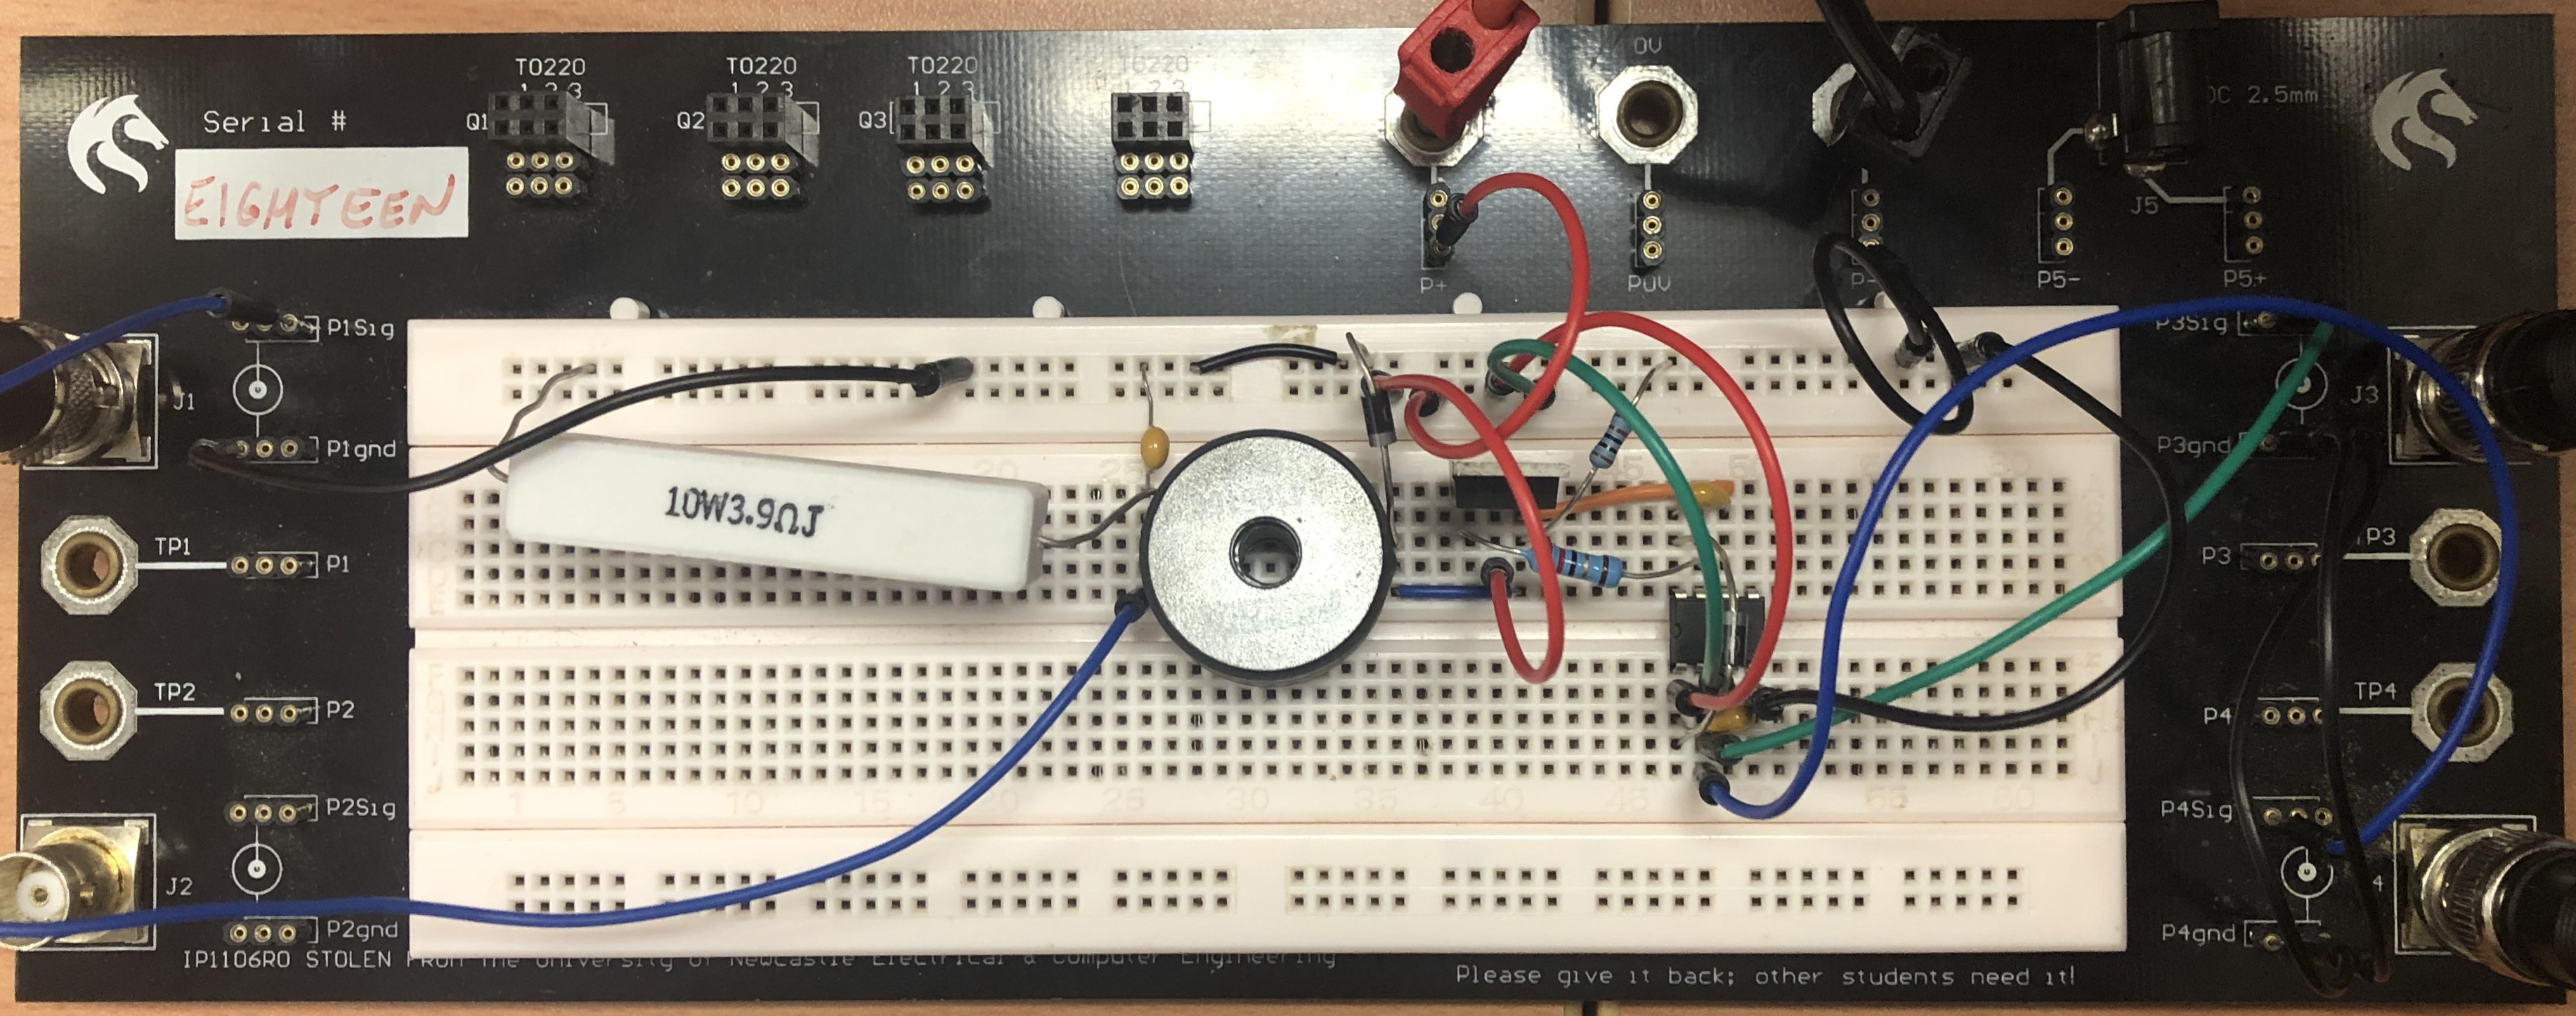
\includegraphics[width=0.7\textwidth]{buck_real}
    \caption{Constructed Buck converter.}
    \label{fig:buck_real}
\end{figure}

\noindent The observed output voltage of the Buck converter for a duty cycle of $D = 62$\% is shown in Figure \ref{fig:buck_expV_newD}. The blue waveform is the output voltage, and the yellow waveform is the PWM input signal to the gate driver. An RMS output voltage of 5.081 V is observed which lies close to the simulated value of 5.0010 V. A peak to peak voltage of 2.000 V is observed which does not align with the simulated ripple voltage of 27.739 mV. This large peak to peak voltage is a result of the large transients that occur when the PWM signal switches. These transients arise from the parasitic inductances of the wires and the parasitic capacitances of the breadboard. As the PWM signal has infinite bandwidth, some of the components of the signal resonant with the parasitic inductances and capacitances which results in large transient responses that are visible in the output waveform. This ripple can only be mitigated through minimizing the parasitic impedances of the device. This could be achieved through designing a printed circuit board (PCB) for the device. This would reduce the parasitic capacitance of the design, as the capacitance formed by the parallel conductive strips on the breadboard would not be present.  The designed PCB would need to feature short trace lengths with tight ground loops to minimize parasitic inductance.\par
\vspace{5mm}
\noindent To explore the output ripple of the converter once the large transients are no longer present, Figure \ref{fig:buck_expV_ripple} displays the steady state output voltage of the Buck converter for $D = 62$\% . A maximum voltage of 5.14 V and a minimum voltage of 5.02 V is observed which results in an output voltage ripple of 120 mV. This output ripple is much larger than the specified ripple of 25 mV and is larger than the simulated ripple of 27.739 mV.  This is likely due to the parasitic inductances of the wires used. This ripple could be reduced through minimizing the length of the wires and by using a larger output capacitor. A larger output capacitor will result in more attenuation of these high frequency ripple components.\par
\newpage
\begin{figure}[h!]
    \centering
    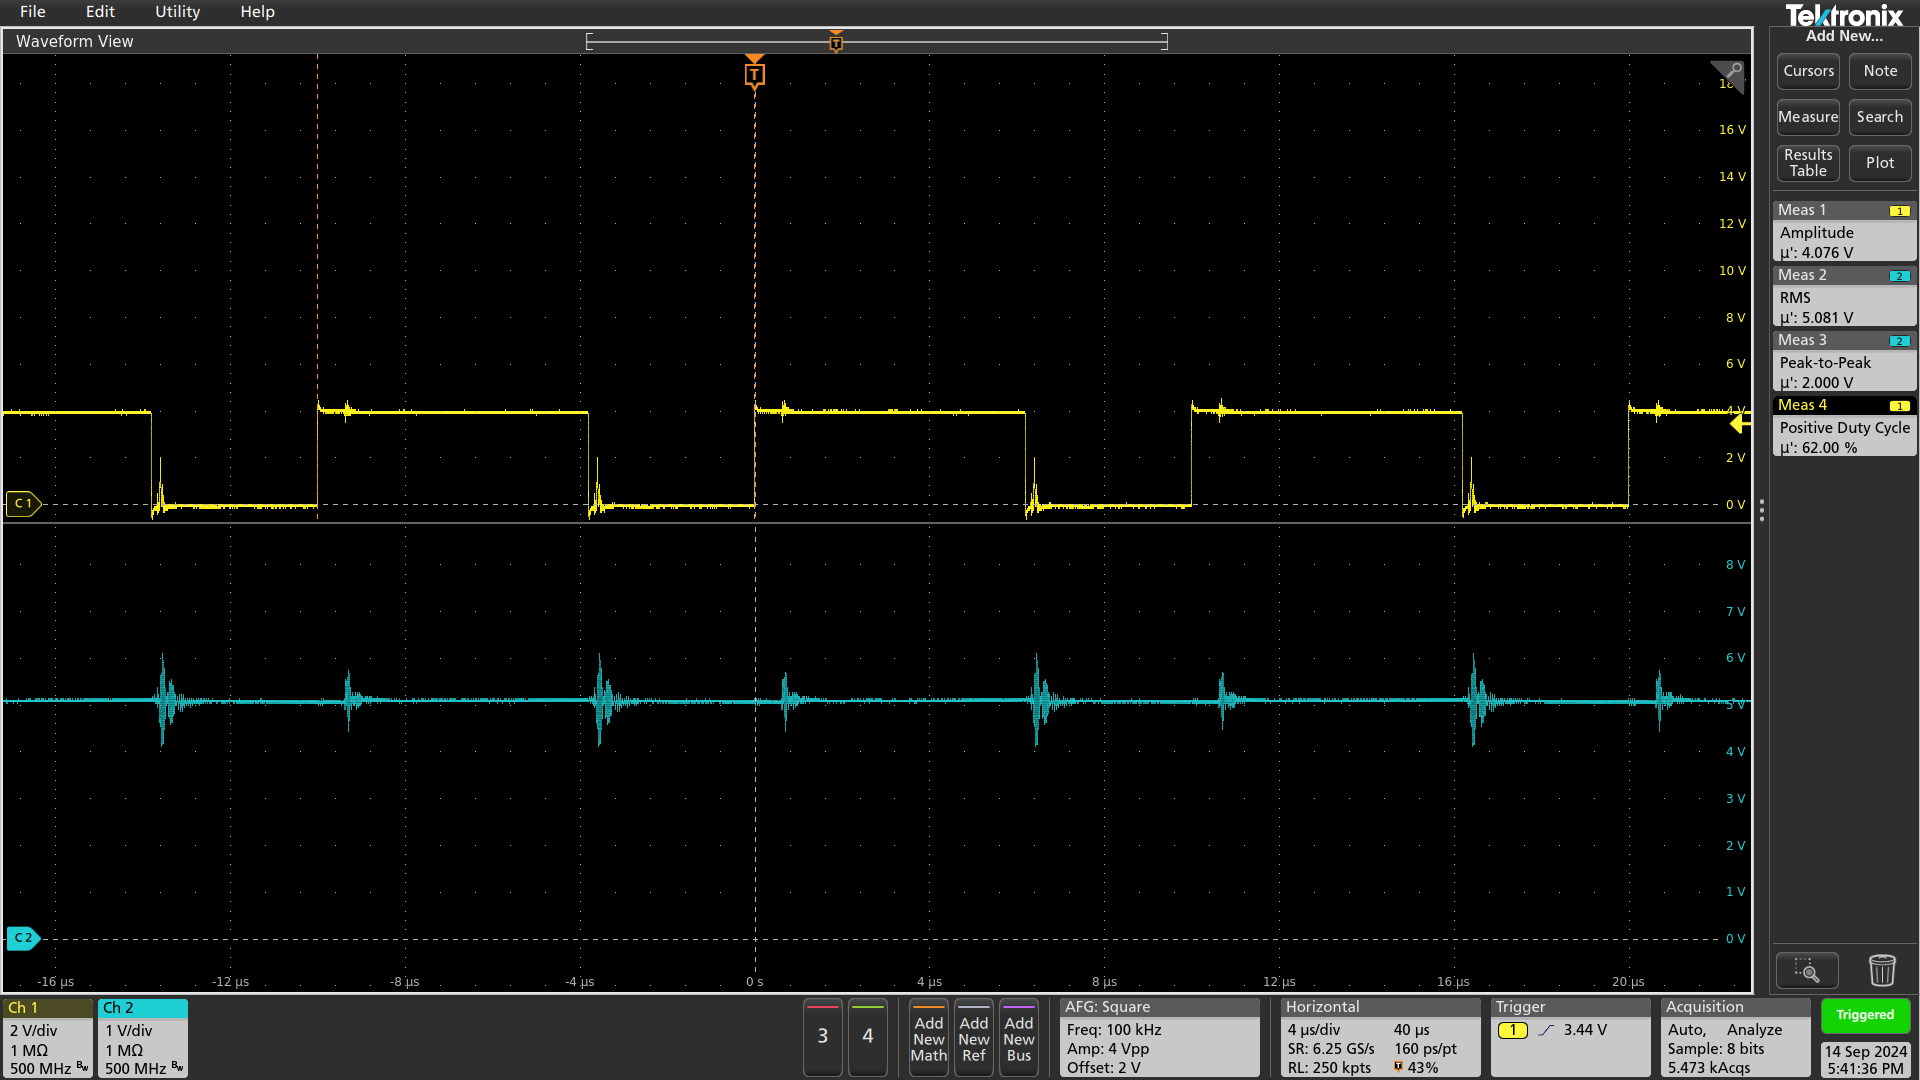
\includegraphics[width=0.7\textwidth]{buck_expV_newD}
    \caption{Output voltage of the Buck converter (blue) for a duty cycle of 62\%. The yellow waveform is the input PWM signal to the gate driver. An RMS voltage of 5.081 V is observed.}
    \label{fig:buck_expV_newD}
\end{figure}
\begin{figure}[h!]
    \centering
    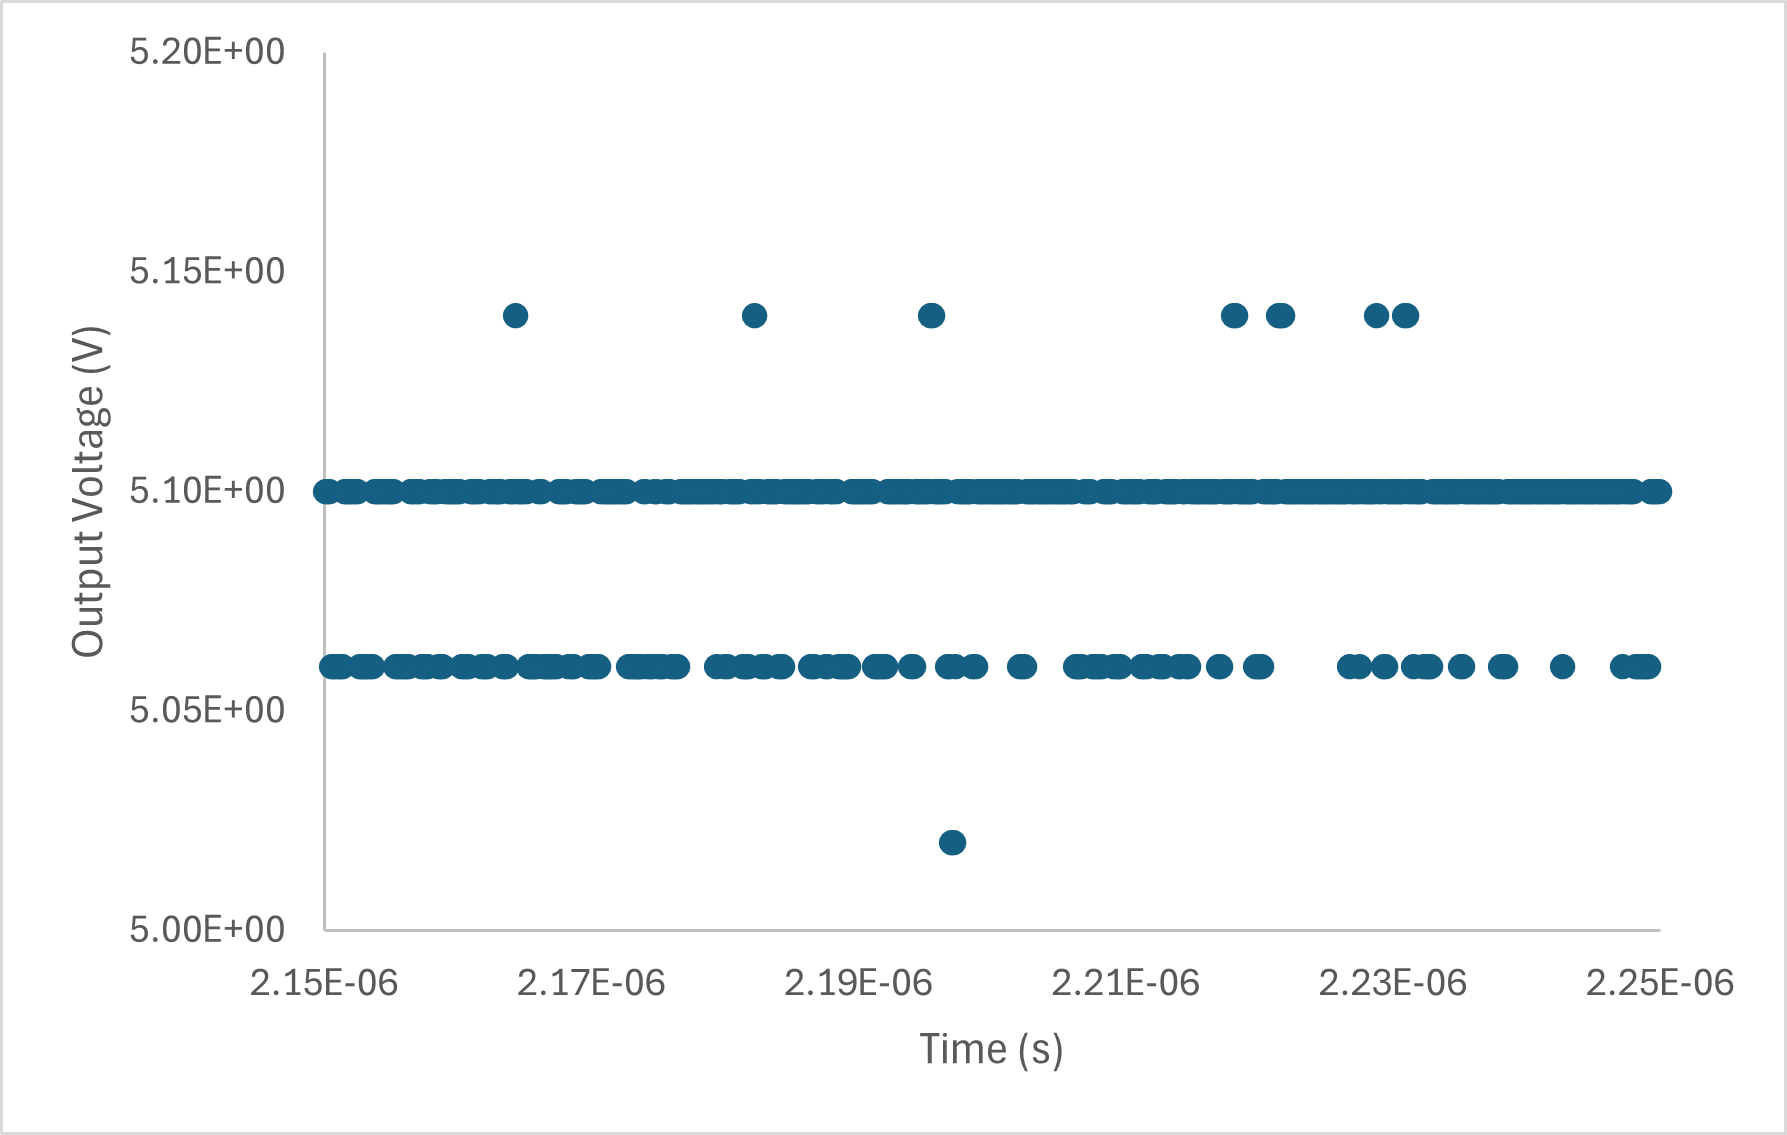
\includegraphics[width=0.7\textwidth]{buck_expV_ripple}
    \caption{Output voltage of the Buck converter in steady state. A ripple voltage of 120 mV is observed.}
    \label{fig:buck_expV_ripple}
\end{figure}

\noindent Figure \ref{fig:buck_expI} displays the inductor current (green waveform) close to the rated output power conditions ($D = 62$\%). An RMS current of 1.11 A is observed which does not agree with the simulated value of 1.2847 A. This is likely a result of the designed converter not accounting for variation in the resistance of the load. This is evidenced by the RMS output voltage (blue waveform) of 4.75 V which implies the load resistance is 4.27 $\Omega$ instead of 3.90 $\Omega$. This was likely not observed in Figure \ref{fig:buck_expV_newD} as the circuit had been running for a longer period of time when the current was measured, compared to when the voltage was measured. This longer operating period likely resulted in the temperature of the load increasing which leads to a larger number of collisions between the electrons and the ions in the load and hence a larger resistance. The dependence of the output voltage on the load could be removed through the use of a closed loop control system with integral action. \par
\vspace{5mm}
\noindent Figure \ref{fig:buck_expI_DCM} (A) displays the inductor (green waveform) for a load of 470 $\Omega$ and $D = 62$\%. The inductor current is observed to reach 0 A but does not remain there for a considerable amount of time, which indicates that the device is on the cusp of DCM. This result aligns with the simulation results. Figure \ref{fig:buck_expI_DCM} (B) displays the inductor current inductor current (green waveform) and output voltage (blue waveform) for a load resistance of 600 $\Omega$. The current spends a larger amount of time near the zero crossing which indicates that the circuit is in DCM mode.

\begin{figure}[h]
    \centering
    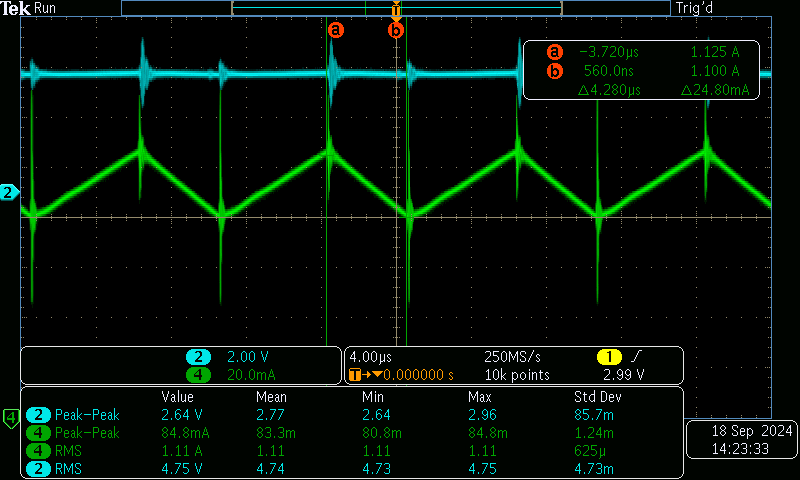
\includegraphics[width=0.7\textwidth]{buck_expI}
    \caption{Output current of the Buck converter under rated power conditions.}
    \label{fig:buck_expI}
\end{figure}

\begin{figure}[h]
    \centering
    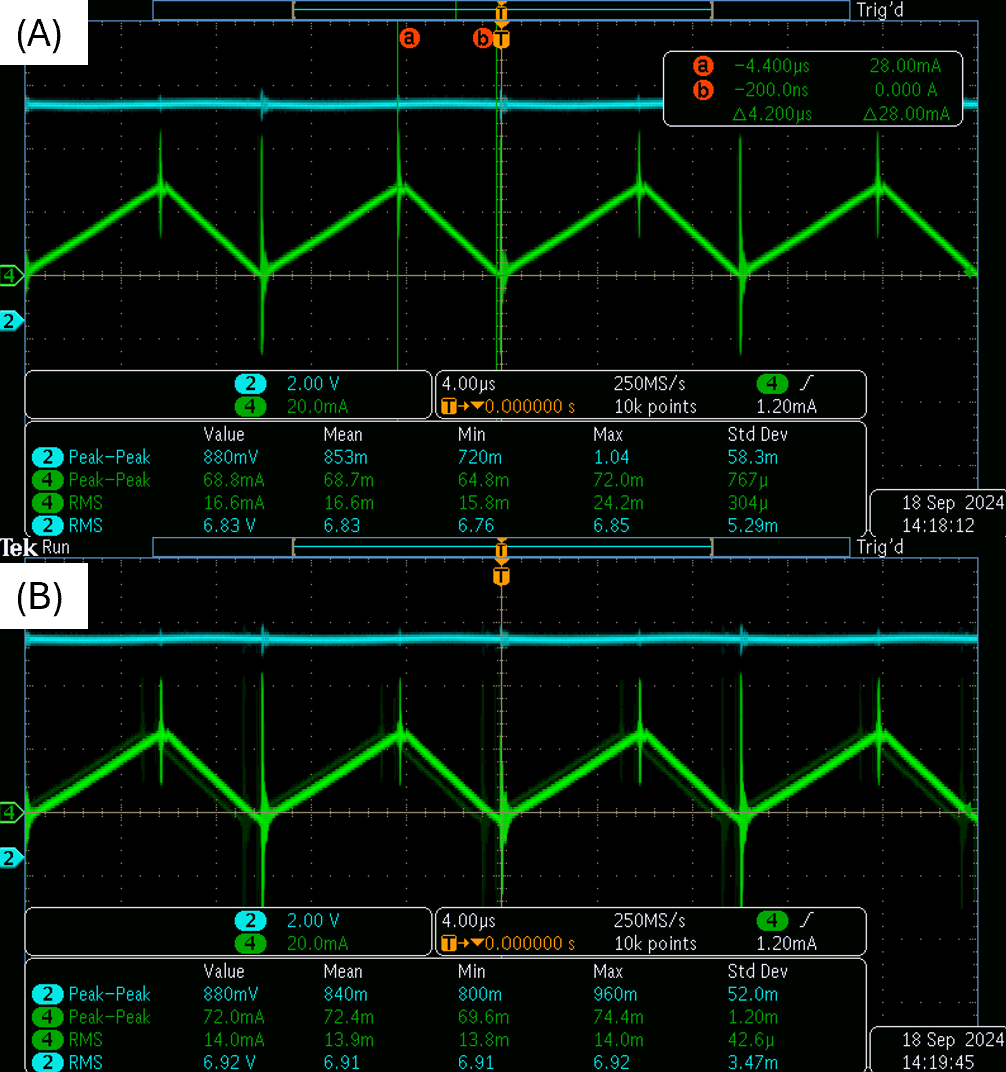
\includegraphics[width=0.7\textwidth]{buck_expI_DCM}
    \caption{Output current of the Buck converter under rated power conditions.}
    \label{fig:buck_expI_DCM}
\end{figure}

\newpage
\section{Flyback Converter}
\citep{BS412-EN}
\citep{jay1995write}
\newpage
\section{Conclusion}
This is blank text.
\newpage
\bibliographystyle{IEEEtranN}
\bibliography{references}

\end{document}
